\begin{figure}[h!]
    \centering
    \caption{Estimated housing expenditure shares}
    \label{fig:hist_housing_exp}

    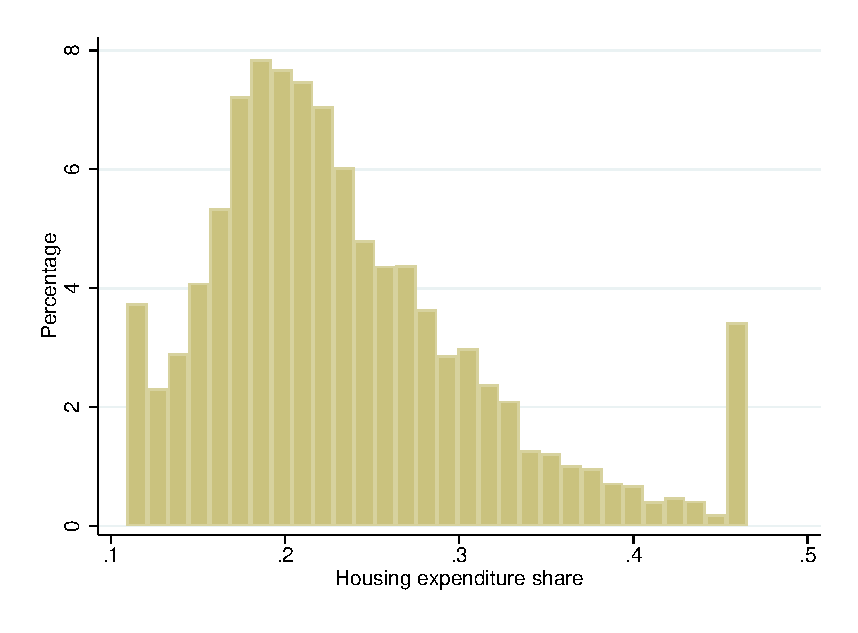
\includegraphics[width = 0.65\textwidth]
            {counterfactuals/output/hist_s_imputed.png}

    \begin{minipage}{.95\textwidth} \footnotesize
        \vspace{3mm}
        Notes: 
        Data are from the \textcite{IRS} and the \textcite{hudSAFMR}.
        The figure shows the ratio between wage per household divided by twelve
        and the SAFMR 40th percentile rent value for a 2-bedroom apartment, both
        for 2018.
        We carry out our computations only for urban ZIP codes, defined as 
        those that belong to a CBSA with at least 80\% of urban population
        according to the 2010 census.
    \end{minipage}
\end{figure}
